\section*{Problemas PI:}

Para os problemas apresentados, realizar:
\begin{enumerate}[label=\alph*)]
    \item Simulação usando MATLAB/Simulink realizando análise dos resultados com relação a estabilidade e 
    resposta dinâmica do sistema
    \item Analisar o LGR sem/com controlador
    \item Determine o tempo de amostragem e realize a discretização dos controladores. Comparar com a
    solução continua.
    \item Discretizar os sistemas (controlador e planta) e analisar a estabilidade usando o método de Jury e
    Routh Hurwitz.
\end{enumerate}
    

\subsection*{Problema 1:}

Para esse problema, o modelo de um motor possui como FT a equação \ref{eq:Gp1}. 

\begin{equation}
    G_p = \frac{4}{s^3+3s^2+10s}
    \label{eq:Gp1}
\end{equation}

A FT de MF, com um controlador proporcional é o visto na equação \ref{eq:Gmf1}.

\begin{equation}
    G_{mf} = \frac{4kp}{s^3+3s^2+10s + 4kp}
    \label{eq:Gmf1}
\end{equation}

Foi visto no desenvolvimento da questão que para o sistema ser estável o ganho propocional deve estar
no intervalo: $0<kp<7,5$. Escolheu-se ter um pólo em -2 e por isso foi determinado $kp = 4$.


\subsubsection*{a)}
    A estabilidade do sistema foi verificada através de uma entrada ao degrau. Pelo desenvolvimento analítico,
    o erro em regime estacionário deve ser zero a uma entrada ao degrau, espera-se obter o mesmo resultado
    pela simulação no MATLAB através do Código \ref{Q1A}.

    \begin{lstlisting}[language=Matlab,label=Q1A,caption=Análise da estabilidade]
%FT sem controlador
num = 4;
den = [1 3 10 0];
G = tf(num,den);
%FT com controlador
kp = 4;
Gmf = tf(kp*num,[1 3 8 4*kp]);

% a)
[y,t] = step(Gmf);
figure
plot(t, y, 'LineWidth', 2);
legend('c(t)')
grid
    \end{lstlisting}

    A Figura \ref{fig:Q1A} apresenta a resposta do sistema ao degrau.


    \begin{figure}[!ht]
        \centering
        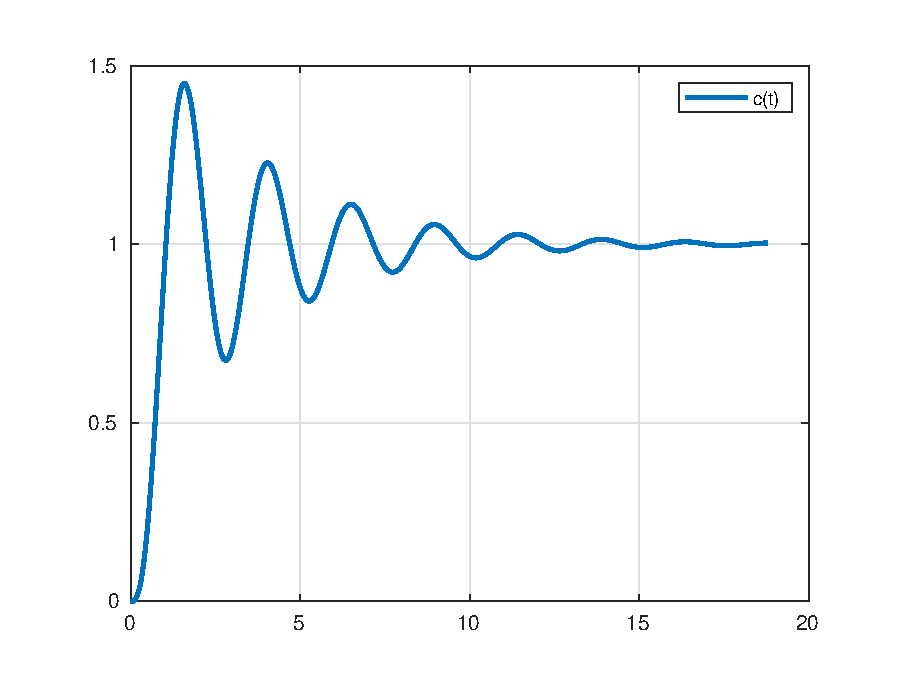
\includegraphics[width = 0.75\linewidth]{Figuras/ProblemasPI/Problema1/step1.eps}
        \caption{Gráfico da resposta ao degrau do sistema}
        \label{fig:Q1A}                   
    \end{figure}

    Podemos verificar que o erro em regime estacionário do sistema tende a zero, assim como determinado 
    através do cálculo analítico. Ainda, podemos verificar que o sistema utilizando um controlador proporcional
    mantém a existência de um sobrevalor percentual.

    Através do \mcode{stepinfo} verifica-se que o sobrevalor percentual é precisamente de 44,93\% e o tempo
    de subida de $T_r =0,6 \text{ s} $. 

\subsubsection*{b)}

    Como já feito anteriormente na avaliação, através da função \mcode{rlocus} é possível traçar o LGR 
    do sistema. A Figura \ref{fig:LGR1Asem} é o LGR do sistema sem o controlador. Pode-se verificar que
    o sistema possui três pólos, com um deles na origem e os outros dois, um par complexo. Como estão 
    no semiplano esquerdo o sistema é estável à resposta ao degrau. Porém o pólo no zero torna o sistema
    mais lento.
    

    \begin{figure}[!ht]
        \centering
        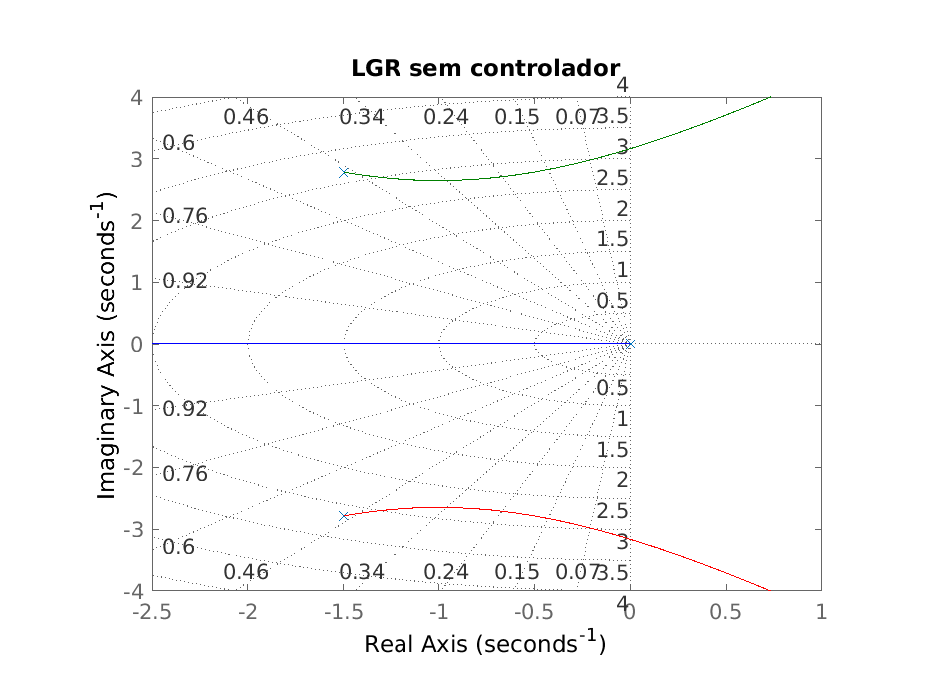
\includegraphics[width = 0.75\linewidth]{Figuras/ProblemasPI/Problema1/LGRsemControlador.eps}
        \caption{Lugar geométrico das raízes sem controlador}
        \label{fig:LGR1Asem}                   
    \end{figure}

    O objetivo do controlador proporcional foi colocar um pólo em -2. Pelo LGR do sistema em MA, o pólo do zero
    é o único que ao variar o ganho se desloca sobre o eixo real. Pode-se verificar através da Figura  
    \ref{fig:LGR1Acom} que o objetivo foi alcançado.

    \begin{figure}[!ht]
        \centering
        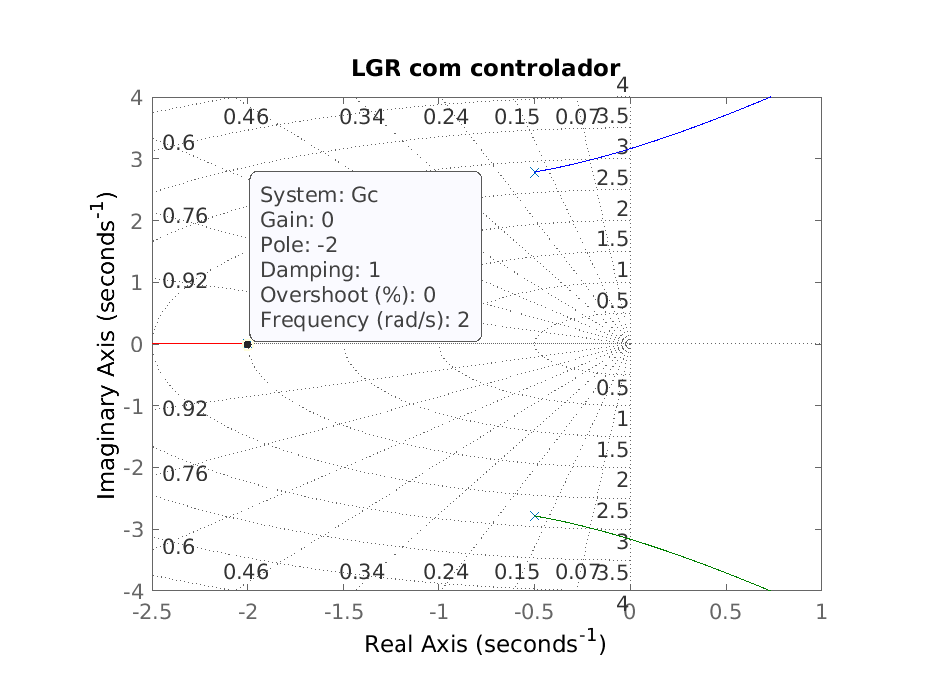
\includegraphics[width = 0.75\linewidth]{Figuras/ProblemasPI/Problema1/LGRcomControlador.eps}
        \caption{Lugar geométrico das raízes com controlador}
        \label{fig:LGR1Acom}                   
    \end{figure}

\newpage    
\subsubsection*{c)}

    Como anteriormente, o tempo de amostragem foi determinado pelo tempo de subida divido por dez. 
    O sistema foi discretizado utilizando o segurador de ordem zero (ZoH). O Código \ref{Q1C} apresenta
    a discretização do modelo e a criação do gráfico da resposta do sistema a entrada degrau.

    \begin{lstlisting}[language=Matlab,label=Q1C,caption=Análise da estabilidade]
Ts = stepinfo(Gmf).RiseTime/10; %Tr = 0.6000
Gmfz = c2d(Gmf,Ts, 'zoh');
[yz,tz] = step(Gmfz); %salvando resultado do step

figure %fazendo uma figura para comparar
plot(t, y, 'LineWidth', 2)
hold on
stairs(tz, yz, 'LineWidth', 2);
hold off
legend('c(t)', 'c(kT)')
grid

%utilizando MAPE para avaliacao numerica
ape = abs((yz - y(1:length(yz)))/y(1:length(yz))); 
mape = mean(ape(isfinite(ape))); %retira o erro percentual do y=0
%mape = 3.2708e-04
    \end{lstlisting}

O tempo de amostragem obtido foi de 60 ms. A FT em MF disceta é apresentada na equação \ref{eq:Gmfz1}
A Figura \ref{fig:Stepctds} apresenta a resposta dos sistema
contínuo e discretizado sobrepostos. 

\begin{equation}
    G_{mf}(z) = \frac{0.0005503 z^2 + 0.002103 z + 0.0005029}{z^3 - 2.807 z^2 + 2.646 z - 0.8353}
    \label{eq:Gmfz1}
\end{equation}


\begin{figure}[!h]
    \centering
    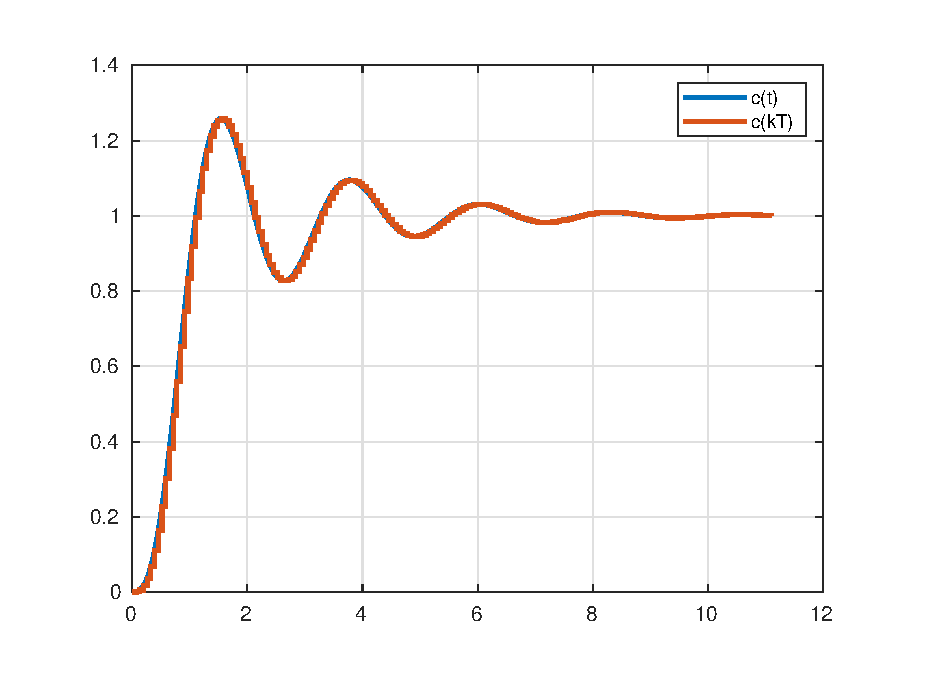
\includegraphics[width = 0.75\linewidth]{Figuras/ProblemasPI/Problema1/resposta_ao_degrau.eps}
    \caption{Lugar geométrico das raízes com controlador}
    \label{fig:Stepctds}                   
\end{figure}

Visualmente o sistema discreto se aproxima da resposta contínua. Porém, como vem sendo feito nessa 
avaliação, verificamos a qualidade da discretização através do MAPE. Para essa discretização o 
MAPE foi de $3,27 \cdot 10^{-2}$ \%. Um baixo valor de erro.

\subsubsection*{d)}

O polinômio característico do sistema contínuo pode ser visto na equação \ref{eq:pcsc1}. O método
de Routh consiste em verificar se há mudança de sinal na primeira coluna da tabela, se não ocorre
o sistema será estável, se ocorrer, instável. A Tabela \ref{tab:RE1} apresenta o desenvolvimento do
resultado obtido 

\begin{equation}
    Q(s) = s^3+3s^2+10s+16
    \label{eq:pcsc1}
\end{equation}

\begin{table}[!ht]
    \centering
    \vspace{0.5cm}
    \caption{Análise de estabilidade pelo método de Routh} 
    \begin{tabular}{r|lr}
        
        1 & 1 & 10 \\
        2 & 3 & 16 \\
        3 & 4{,}67\\
    \end{tabular}                
    \label{tab:RE1}
\end{table}

Verificamos que o sistema contínuo é estável.

O polinômio característico do sistema discreto pode ser visto na equação \ref{eq:pcsd1}.

\begin{equation}
    Q(z) = z^3 - 2.807 z^2 + 2.646 z - 0.8353
    \label{eq:pcsd1}
\end{equation}

A Tabela \ref{tab:JE1} apresenta o desenvolvimento do método de Jury para esse sistema.

\begin{table}[!ht]
    \centering
    \caption{Análise de estabilidade} 
    \begin{tabular}{l| r r r r}
         & $z^0$ & $z^1$ & $z^2$ & $z^3$\\
        \hline
        1 & -0{,}8353 & 2{,}646 & -2{,}807 & 1\\
        2 & 1 & -2{,}807 & 2{,}646 & -0{,}8353\\
        3 & -0{,}3013 & 0{,}5968 & -0{,}3023 & 0\\
    \end{tabular}                
    \label{tab:JE1}
\end{table}

Para verificar a estabilidade, como nosso polinômio é de ordem 3, devemos conferir os 4 critérios.

- O primeiro critério: $Q(1)= 3,7 \cdot 10^{-3} > 0$, satisfeito; \\
- O segundo critério: $-1^3 Q(-1) = 7,2883 > 0$, satisfeito;\\
- O terceiro critério: $|a_0| = 0,8353 < 1 = |a_3|$, satisfeito; \\
- O quarto critério: $|b_0| = 0,3023 > 0,3408 = |b_3| $, satisfeito. 

Como o sistema discreto atende os quatro critérios de Jury necessários, é um sistema estável.

\subsection*{Problema 2:}